%#MAKEINDEX makeindex interim01
\documentclass[10pt,a4j]{jarticle}

\input{include/macro.tex}
\input{include/preamble.tex}

\begin{document}
%%%%%%%%%%%%%%%%%%%%%%%%%%%%%%%%%%%%%%%%%%%%%%%%%%%%%%%%%%%%%%%%%%%%%%
\section{消火用機構}
消火方法は前述の通りであるが,ここではそのための機構であるアーム機構について述べる.
アームは垂直方向に上下する1リンク機構を考える.これは,消火方法が布を押し込むという単純なものであるためである.

\begin{figure}[h]
 \centering
 \begin{tabular}{c}
  
  \begin{minipage}{0.3\hsize}
   \centering
   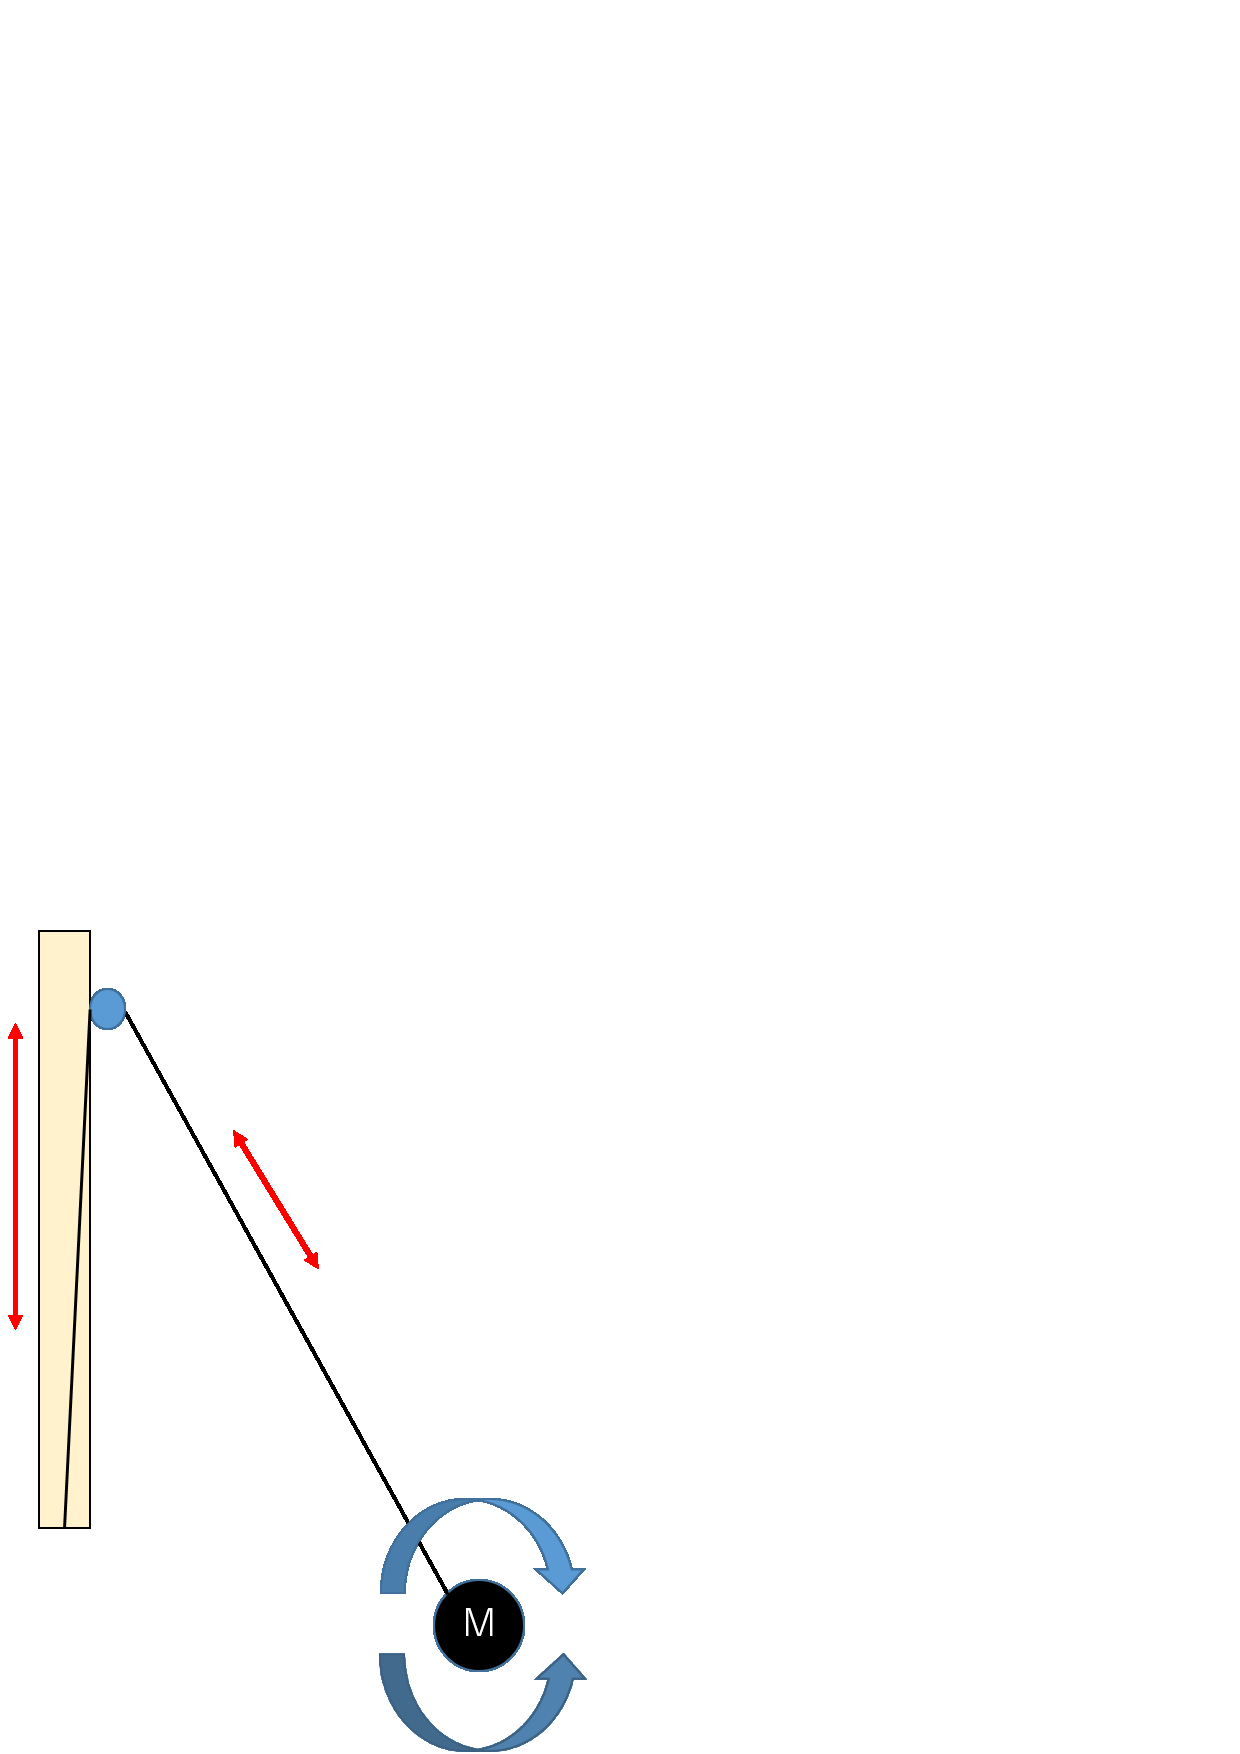
\includegraphics[clip,scale=0.3]{./picture/arm_img.png}
   \hspace{1cm} [1]アーム概念図
  \end{minipage}
  
  \begin{minipage}{0.45\hsize}
   \centering
   \includegraphics[clip,scale=0.05]{./picture/arm_real.png}
   \hspace{1.6cm} [2]製作したアーム
  \end{minipage}
 \end{tabular}
 \caption{消火用アーム}
 \label{arm}
\end{figure}





%%%%%%%%%%%%%%%%%%%%%%%%%%%%%%%%%%%%%%%%%%%%%%%%%%%%%%%%%%%%%%%%%%%%%%%%%%%%
\end{document}